\documentclass[conference,a4paper]{IEEEtran}
\usepackage[T1]{fontenc}
\usepackage{graphicx,booktabs,amsmath,amssymb,siunitx,multirow,xcolor}
\usepackage{tikz}
\usetikzlibrary{arrows.meta,angles,quotes,decorations.pathmorphing,calc}
\usepackage[hidelinks]{hyperref}
\usepackage{cite}
\graphicspath{{../figures/}}
\sisetup{detect-all}
\DeclareSIUnit[number-unit-product = {}]\degree{\ensuremath{^\circ}}
\newcommand{\degr}{\ensuremath{^\circ}}

\begin{document}

\title{Where Does the Chip Go?\\ Phone-Based Monitoring of Chip Flow,\\ Chip Ejection and Entanglement in CNC Turning}

% TODO: replace with the group members' names and the institute
\author{\IEEEauthorblockN{ME361 Project Group}
\IEEEauthorblockA{Department of Mechanical Engineering\\
Course project report, November 2026}}

\maketitle

\begin{abstract}
Long continuous chips that wrap around the tool and the workpiece are a common problem in finish turning.
We study whether an ordinary smartphone, held above the tool, can measure where the chip goes and warn when chips start to entangle.
Six dry outer-diameter cuts on mild steel were filmed from the top at two feeds (0.08 and \SI{0.15}{mm/rev}) and three depths of cut (0.3, 0.6 and \SI{0.9}{mm}) at a constant cutting speed of \SI{150}{m/min}.
We separate two angles that are often confused: the \emph{chip-flow angle} on the rake face, which classical theory predicts, and the \emph{ejection direction} of the chip in the air, which decides where chips land and tangle.
The ejection direction, measured frame by frame, increases with feed in all 18 analysis variants tried, and lies \SIrange{72}{105}{\degree} away from the rake-face direction predicted by Colwell's model.
A second measurement, based on the standing image of the chip on the insert, finds the rake-face flow on the insert side of the tip as theory predicts; on the clearest run it agrees with Colwell's model when the nose radius is taken as \SIrange{0.8}{1.2}{mm}.
A linear model of feed and depth predicts the run-level ejection angle with a leave-one-run-out error of \SI{6.6}{\degree} (baseline \SI{7.9}{\degree}).
Cutting runs into sub-clips helps only modestly, and a random frame split reports errors as low as \SI{0.05}{\degree} that are pure leakage.
For image networks, a label-changing rotation augmentation reduces the squeezing of predictions only when it rotates the motion channels alone. No image model clearly beats the linear model, and none transfers to earlier footage of a different cut.
The phone microphone gives spindle speed within 0.4\% and feed within 2.6\%, and a training-free indicator raises an alarm only on the one run where chips tangled.
Everything runs live in a browser-based demonstrator.
\end{abstract}

\begin{IEEEkeywords}
chip flow angle, chip control, turning, machine vision, condition monitoring, data leakage, smartphone sensing
\end{IEEEkeywords}

\section{Introduction}
Chip control is a practical limit in turning: long, unbroken chips snarl around the tool and the part, scratch the finished surface, can chip the insert and force the operator to stop the machine \cite{jawahir1993}.
Published chip monitoring mostly uses force or acoustic-emission (AE) sensors \cite{dornfeld1985,sukvittayawong1991,kishawy2018}.
These work well but are not found on the average teaching or job-shop lathe.
This project asks how far a smartphone can go, using its camera and microphone, with no fixture beyond a hand or a clamp.

The work makes five contributions:
\begin{enumerate}
\item a frame-by-frame measurement of the chip \emph{ejection} direction from top-view video, with a sensitivity analysis of its settings;
\item a separate measurement of the chip flow on the \emph{rake face} from the standing image of the chip, which resolves an apparent conflict with chip-flow theory;
\item a leave-one-run-out comparison of eleven settings-to-angle models, a test of the sub-clip ("more data") idea, and a demonstration of how random splits leak;
\item image models with a label-changing rotation augmentation, and a test on earlier footage taken under different conditions;
\item two applications of the same recording: a sound-based virtual sensor for spindle speed and feed, and a training-free chip build-up alarm, both shown live in a browser demonstrator.
\end{enumerate}

\section{Two angles: flow on the rake face and ejection}\label{sec:angles}
The \emph{chip-flow angle} $\eta$ is defined on the rake face.
For a straight oblique edge, Stabler's rule states that the chip flows across the rake face at an angle to the normal of the cutting edge roughly equal to the inclination angle \cite{stabler1951}.
For a tool with a nose radius, the engaged edge is curved.
Colwell \cite{colwell1954} takes the flow as perpendicular to the chord that joins the two ends of the engaged edge.
Young, Mathew and Oxley (YMO) \cite{young1987} add up the edge normals weighted by the chip area each element removes.
In both models $\eta$ grows when the depth of cut $a_p$ is small compared with the nose radius $r_\varepsilon$, because the curved nose then makes up a larger share of the engaged edge.
Feed has only a small effect.

What a camera sees a few millimetres from the tip is different.
The chip leaves the rake face, curls up and sideways, may hit the chip breaker or the shoulder of the part, and then flies off.
We call the direction in which it leaves the cutting zone the \emph{ejection direction} $\psi$.
It decides where chips land and whether they wrap around the tool, but no closed-form model predicts it.

\begin{figure}[t]
\centering
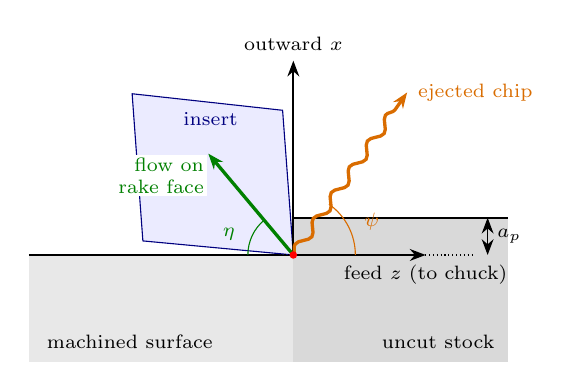
\begin{tikzpicture}[scale=1.05,>={Stealth[length=2mm]}]
  % workpiece, top view: machined surface below the tip, uncut stock (ap) to the right
  \fill[gray!18] (-3.2,-1.3) rectangle (0,0);
  \fill[gray!30] (0,-1.3) rectangle (2.6,0.45);
  \draw[thick] (-3.2,0) -- (0,0) -- (0,0.45) -- (2.6,0.45);
  \node[font=\scriptsize,anchor=west] at (-3.1,-1.05) {machined surface};
  \node[font=\scriptsize,anchor=east] at (2.55,-1.05) {uncut stock};
  \draw[<->,thin] (2.35,0) -- (2.35,0.45) node[midway,right,font=\scriptsize]{$a_p$};
  \draw[densely dotted] (0,0) -- (2.2,0);
  % insert (rhombic, rake face up)
  \filldraw[fill=blue!8,draw=blue!50!black] (0,0) -- (-0.13,1.75) -- (-1.95,1.95) -- (-1.82,0.17) -- cycle;
  \node[font=\scriptsize,blue!50!black] at (-1.0,1.65) {insert};
  % axes
  \draw[->,thick] (0,0) -- (1.6,0) node[below,font=\scriptsize]{feed $z$ (to chuck)};
  \draw[->,thick] (0,0) -- (0,2.35) node[above,font=\scriptsize]{outward $x$};
  % rake-face flow and ejection
  \draw[->,very thick,green!50!black] (0,0) -- ({1.6*cos(130)},{1.6*sin(130)}) node[below left,font=\scriptsize,align=right,fill=white,inner sep=1pt]{flow on\\ rake face};
  \draw[->,very thick,orange!85!black,decorate,decoration={snake,amplitude=0.6mm,segment length=4mm,post length=2mm}] (0,0) -- ({2.4*cos(55)},{2.4*sin(55)}) node[right,font=\scriptsize]{ejected chip};
  % angle arcs
  \draw[orange!85!black] (0.75,0) arc (0:55:0.75); \node[font=\scriptsize,orange!85!black] at (0.95,0.4) {$\psi$};
  \draw[densely dotted] (0,0) -- (-1.4,0);
  \draw[green!50!black] (-0.55,0) arc (180:130:0.55); \node[font=\scriptsize,green!50!black] at (-0.78,0.25) {$\eta$};
  \fill[red] (0,0) circle (1.3pt);
\end{tikzpicture}
\caption{The two angles in the top view used throughout. The camera looks down on the rake face, so the image is close to the tool reference plane. $\psi$ is measured from the feed direction towards radially outward. The flow-angle theory gives $\eta$ from straight back over the insert towards outward, so the rake-face flow points at $\psi_\mathrm{face}=180\degr-\eta$. Values drawn are the measured ones for run R2.}
\label{fig:angles}
\end{figure}

With the camera above the tool, the image plane is nearly the tool reference plane and the rake face is seen face-on.
Both angles can therefore be written in one convention (Fig.~\ref{fig:angles}): $\psi$ is measured from the feed direction (towards the chuck) to radially outward.
The rake-face flow predicted by theory points at $\psi_\mathrm{face}=180\degr-\eta$.
For our runs, theory puts $\psi_\mathrm{face}$ at \SIrange{122}{157}{\degree}, which is on the insert side of the tip.
The first iteration of this project compared theory with $\psi$ and found the opposite trend (Section~\ref{sec:res-face}).
The main new result here is that the two angles have to be measured separately.

\section{Experiments}
\subsection{Cutting tests}
Six dry outer-diameter turning passes towards the chuck were made on a CNC lathe with a FANUC 0i Mate-TD controller, on a mild steel bar (grade not recorded, taken as AISI 1020).
The program used G96 constant surface speed at $V_c=\SI{150}{m/min}$ and cut a length of \SI{61}{mm}.
The insert code was not recorded.
The videos show a screw-clamped insert with a moulded chip breaker, and we assume a CCMT 09T304 ($r_\varepsilon=\SI{0.4}{mm}$, \SI{80}{\degree} rhombus) in a \SI{95}{\degree} holder.
Section~\ref{sec:res-face} shows that the nose radius is probably larger.
Table~\ref{tab:runs} lists the runs.
Because the bar diameter shrank from run to run, the spindle speed rose with run order.

\begin{table}[t]
\caption{Cutting runs (order R1--R6). Frames: valid frames in the steady part of the cut.}
\label{tab:runs}
\centering\small
\begin{tabular}{@{}lcccrr@{}}
\toprule
Run & $f$ (mm/rev) & $a_p$ (mm) & $D$ (mm) & rpm & Frames \\
\midrule
R1 & 0.08 & 0.9 & 32.0$\to$30.2 & 1581 & 690 \\
R2 & 0.15 & 0.9 & 30.2$\to$28.4 & 1681 & 241 \\
R3 & 0.08 & 0.3 & 28.4$\to$27.8 & 1717 & 499 \\
R4 & 0.15 & 0.3 & 27.8$\to$27.2 & 1755 & 253 \\
R5 & 0.08 & 0.6 & 27.2$\to$26.0 & 1836 & 418 \\
R6 & 0.15 & 0.6 & 26.0$\to$24.8 & 1925 & 235 \\
\bottomrule
\end{tabular}
\end{table}

\subsection{Recording}
A phone was held above the tool and followed it along the cut.
It recorded 1920$\times$1080 pixels at 30 frames/s, with sound.
A second, side-view recording was too far away to show chips and is not used.
For an out-of-domain test we also used footage from an earlier visit (October 2026).
It shows a different, stepped part cut near the tailstock, at unknown settings, in 15 clips recorded at 60 frames/s while the user zoomed in and out.

\section{Methods}
\subsection{Ejection direction $\psi$}\label{sec:m-eject}
Each frame is scaled to \SI{960}{px} on its long side.
The insert is tracked by normalised template matching ($120\times120$ px template, $\pm90$ px search window).
The workpiece axis is re-estimated in every frame from long straight Hough lines, which removes phone rotation.
Moving pixels are found by three-frame differencing after the neighbouring frames are shifted by the tip motion, keeping the smaller of the two differences above a threshold of 18 grey levels.
Within an annulus of \SIrange{25}{220}{px} around the tip, the motion-weighted histogram of pixel directions (2\degr\ bins, Gaussian smoothing) is formed, and its peak is $\psi$ for that frame.
Each frame also gives the spread of the directions (circular SD), the mean reach, the moving area, and the edge density of static chips in front of the tool (clutter).
Of 3,142 frames, 2,336 are valid and lie in the steady part of a cut.

\subsection{Flow on the rake face}\label{sec:m-face}
On the rake face the chip slides along itself at roughly the chip velocity ($\approx$\SI{1}{m/s}), so frame differencing barely sees it.
Seen at 30 frames/s it is a \emph{standing} bright band, while flying chips come and go.
The method has four steps:
\begin{enumerate}
\item From every native-resolution frame of the steady cut, cut a $280\times280$ px crop around the tracked tip, rotated so that the feed points right.
\item Take the temporal median of these crops. This keeps the insert and the standing chip and removes flying chips.
\item Subtract a chip-free reference of the same insert. Frames before and after the cut cannot serve, because there the tool is off the bar. The reference is therefore the median of the other five runs' standing images, each registered to this run with an affine enhanced-correlation-coefficient fit \cite{evangelidis2008} on the insert pattern away from the tip.
\item In the positive difference image, find the direction from the tip whose 9-px-wide ray (0.5--\SI{3.3}{mm}) has the highest mean contrast on the insert side ($95\degr\le\psi\le175\degr$). Beyond \SI{175}{\degree} the ray runs along the bar edge.
\end{enumerate}
This is repeated in 1-s windows.
A window counts as a detection when its peak is more than 2 SD above the median over all rays.

\subsection{Settings-to-angle models and evaluation}\label{sec:m-models}
With six runs, the only honest test is leave-one-run-out (LORO): fit on five runs, predict the sixth, repeat.
Frames from one run are strongly correlated.
Any split that puts frames of the test run into training lets a model look the answer up; this is the leakage pattern described by Kapoor and Narayanan \cite{kapoor2023}.
We report the run-level RMSE of the predicted mean angle and compare it with predicting the training mean.

\subsection{Image models}\label{sec:m-cnn}
For every valid frame a $224\times224$ crop is cut so that the tip sits at (35\%, 65\%) of the crop, the feed points right and outward points up.
The label is the 0.5-s rolling median of $\psi$.
All networks are ImageNet-pretrained ResNet-18 \cite{he2016}, fine-tuned for 8 epochs and scored by LORO.
They differ in input and augmentation:
\begin{itemize}
\item \textbf{RGB} (v1): the plain crop.
\item \textbf{Motion} (v2): the three channels are [grey, $|$difference to the previous frame$|$, $|$difference to the next frame$|$]. The tool is static in the crop, so only chips light up.
\item \textbf{Motion + rotation} (v3, new): the crop is rotated about the tool tip by $\delta\sim U(-35\degr,35\degr)$ and the label becomes $\psi+\delta$. Because the crop axes are fixed to the feed direction, this creates chip directions the six runs never produced, without inventing a cut.
\item \textbf{Clip + rotation} (v3, new): five frames are stacked as [grey, $|d_{t-2}|$, $|d_{t-1}|$, $|d_{t+1}|$, $|d_{t+2}|$].
\item \textbf{Histogram + ridge}: no network. A 216-bin histogram of motion directions (72 angles by 3 radii) is fed to a ridge regression.
\end{itemize}

\subsection{Sound}
\textbf{Spindle speed.} A harmonic-sum pitch search (8 harmonics, 2-s windows, 0.5-s hop) gives the spindle speed.
\textbf{Cutting state.} The 2--\SI{6}{kHz} band level rises by more than \SI{5.5}{dB} over idle while cutting.
\textbf{Feed.} With a known cut length $L$, feed is $f=L/(t_\mathrm{cut}\,n)$.

\subsection{Build-up indicator}
The indicator needs no training.
Three signals are converted into robust $z$-scores against the first \SI{4}{s} of the same cut:
\begin{itemize}
\item $\log$ moving area;
\item spray spread;
\item static clutter.
\end{itemize}
The alarm is raised when the 1-s rolling median of their mean stays above 3 for \SI{1}{s}.

\subsection{Live demonstrator}
A laptop server (Python, Starlette over HTTPS and websockets) receives JPEG frames and 16-kHz audio from a phone's browser.
It runs a causal version of the same per-frame code and serves a dashboard.
The dashboard has four steps:
\begin{enumerate}
\item cutting parameters, with the model prediction;
\item calibration: three clicks for tip, feed and outward, plus an idle-sound check of spindle speed;
\item live view;
\item summary.
\end{enumerate}
A replay mode runs the recorded runs through identical code.

\section{Results}
\subsection{Ejection direction}
The chip leaves the tip at $\psi\approx$\SIrange{42}{62}{\degree} (Table~\ref{tab:eject}), forward and outward.
The frame-to-frame SD is \SIrange{15}{20}{\degree}.
Raising the feed from 0.08 to \SI{0.15}{mm/rev} increases $\psi$ at every depth (+10.1, +8.4, +\SI{2.7}{\degree}).
The sign of this effect is the same in all 18 combinations of annulus radius (150/220/300 px), motion threshold (12/18/28) and estimator (histogram peak or weighted mean).
The annulus radius shifts all runs together by \SIrange{3}{6}{\degree}: further out, the chip has curved more.
The absolute value of $\psi$ therefore depends on where it is taken; the differences between runs do not.
An estimator based on the orientation of motion streaks failed (SD 40--\SI{50}{\degree}), because at 30 frames/s chips appear as blobs, not streaks.
The angle also drifts upward during a cut (by up to \SI{27}{\degree} in R5).

\begin{table}[t]
\caption{Measured directions (deg). $\psi$: ejection, mean with bootstrap 95\% CI. $\psi_\mathrm{face}$: rake face, median over 1-s windows (detected/total windows). Theory: Colwell, $\psi_\mathrm{face}=180-\eta$, for $r_\varepsilon=0.4$/\SI{0.8}{mm}.}
\label{tab:eject}
\centering\small
\setlength{\tabcolsep}{4pt}
\begin{tabular}{@{}lcccc@{}}
\toprule
Run & $\psi$ (CI) & $\psi_\mathrm{face}$ (det.) & Theory & $\eta$ meas./theory \\
\midrule
R1 & 51.5 (49--53) & --- (0/23) & 157/138 & --- \\
R2 & 61.7 (59--65) & \textbf{129} (8/9) & 154/136 & \textbf{51}/26/44 \\
R3 & 41.8 (39--45) & 110 (10/19) & 125/114 & 70/55/66 \\
R4 & 50.2 (47--54) & 139 (1/9) & 122/113 & --- \\
R5 & 43.3 (40--47) & 112 (2/14) & 145/126 & --- \\
R6 & 45.9 (44--48) & 129 (4/7) & 142/125 & 52/38/55 \\
\bottomrule
\end{tabular}
\end{table}

\subsection{Flow on the rake face}\label{sec:res-face}
\begin{figure}[t]
\centering
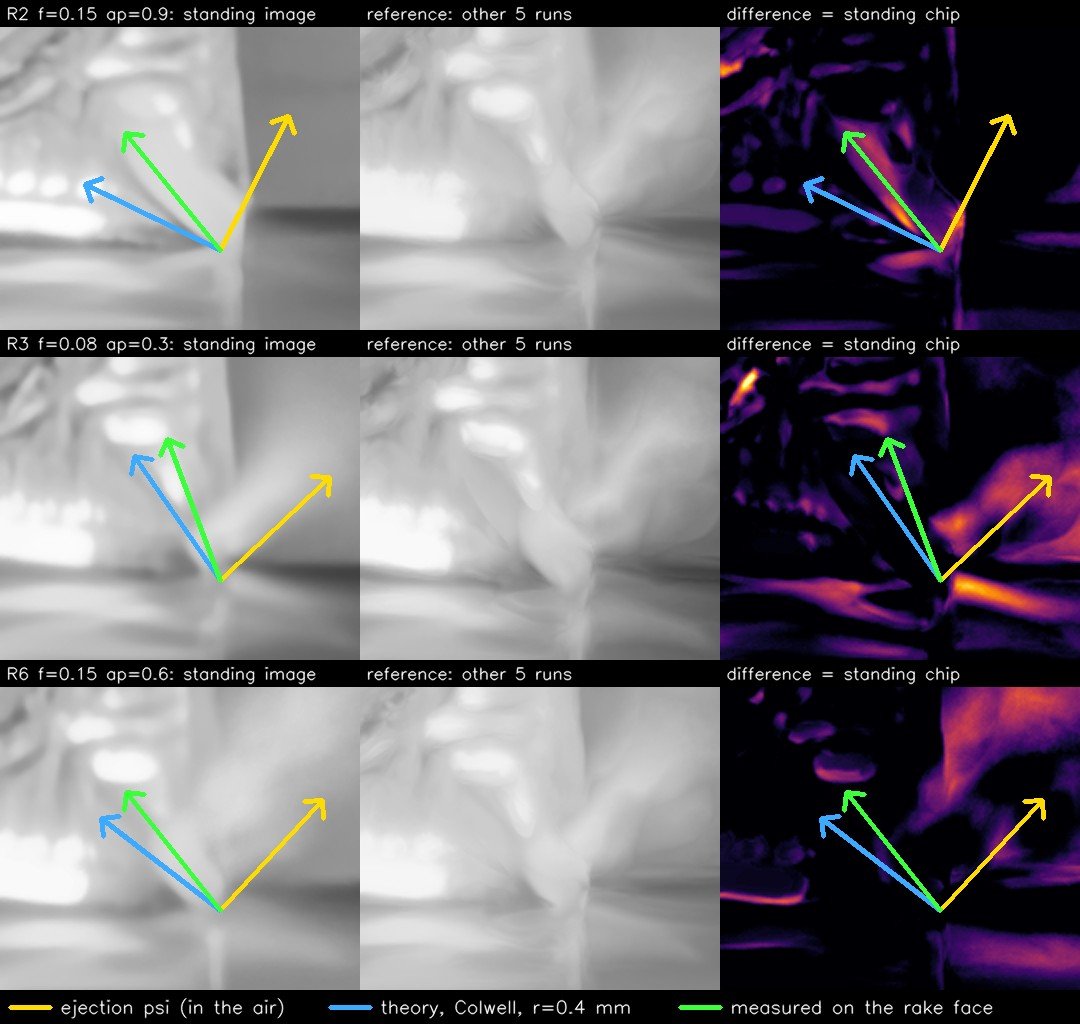
\includegraphics[width=\columnwidth]{fig12_rake_face.jpg}
\caption{Standing image of the chip at full resolution, tip-centred, feed to the right. Left: temporal median over the steady cut. Middle: the other five runs registered onto it. Right: difference, which shows the standing chip. Arrows: ejection $\psi$ (yellow), Colwell theory for $r_\varepsilon=\SI{0.4}{mm}$ (blue), measured rake-face direction (green). In R2 the chip band on the insert is clear; in R3 and R6 it is faint.}
\label{fig:face}
\end{figure}

\begin{figure}[t]
\centering
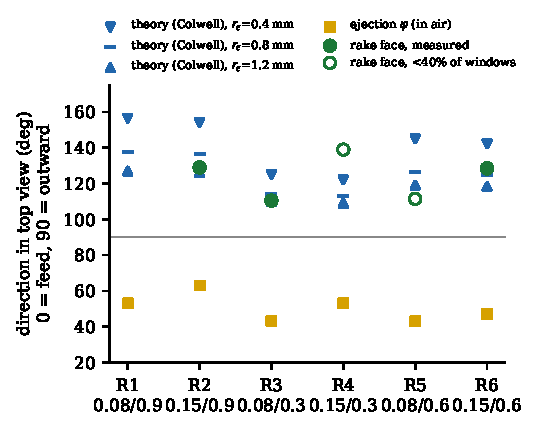
\includegraphics[width=\columnwidth]{fig13_rake_vs_theory.pdf}
\caption{Ejection (squares) and rake-face (circles) directions compared with Colwell's flow direction for three nose radii. On the rake face the chip goes to the insert side ($\psi>90\degr$), as theory says. In the air it goes forward.}
\label{fig:face-theory}
\end{figure}

Figs.~\ref{fig:face} and~\ref{fig:face-theory} and Table~\ref{tab:eject} give the result.
On the deepest cuts, R1 and R2 with $a_p=\SI{0.9}{mm}$, a bright standing band runs from the tip across the insert, up and back.
In R2 the band is found in 8 of 9 one-second windows at $\psi_\mathrm{face}=\SI{129}{\degree}$ (interquartile range 129--130), i.e.\ $\eta=\SI{51}{\degree}$.
In R1 the band is visible in the raw crops but the detector does not lock on it reliably, so no value is reported.
For the shallower cuts the chip is narrow (0.3--\SI{0.6}{mm}, i.e.\ 9--18 native pixels) and leaves the face quickly.
R3 and R6 give weaker detections (10/19 and 4/7 windows) at 110\degr\ and 129\degr; R4 and R5 give no stable value.

The key finding is the side of the tip on which the chip lies.
Every detected rake-face direction lies on the insert side, \SIrange{110}{129}{\degree}, where theory puts it.
The ejection directions lie on the other side of the outward normal, at \SIrange{42}{62}{\degree}.
The negative correlation between theory and measurement reported in our first iteration (\mbox{$r=-0.52$}) is therefore a property of the \emph{ejection}: it does not show that flow-angle theory fails.

The size of $\eta$ fits a larger nose radius than we assumed.
For R2, Colwell's model gives $\eta=26\degr$, 44\degr\ and 54\degr\ for $r_\varepsilon=0.4$, 0.8 and \SI{1.2}{mm}; the measurement is \SI{51}{\degree}.
Fitting $r_\varepsilon$ to the three detected runs gives the lowest error at \SIrange{0.8}{1.0}{mm} (RMSE \SIrange{5.1}{4.4}{\degree}), against \SI{18.5}{\degree} for the assumed \SI{0.4}{mm}.
The YMO model needs $r_\varepsilon\approx\SI{1.2}{mm}$.
Since R3 and R6 are weak detections, this is an estimate of the insert's nose radius to be checked on the insert, not a validation of either model.

\subsection{Settings-to-angle models and the "more data" question}
\begin{table}[t]
\caption{Settings-to-ejection-angle models, LORO on run means (deg).}
\label{tab:zoo}
\centering\footnotesize
\begin{tabular}{@{}lcc@{}}
\toprule
Model & RMSE & MAE \\
\midrule
Linear $f+a_p+\text{rpm}$ (confounded with run order) & 4.6 & 3.9 \\
Random forest ($f$, $a_p$) & 6.5 & 5.6 \\
\textbf{Linear $f+a_p$} & \textbf{6.6} & \textbf{5.8} \\
Ridge with $f\cdot a_p$ & 7.0 & 5.9 \\
$k$-NN ($k=2$) & 7.6 & 6.4 \\
Quadratic ridge & 7.9 & 6.7 \\
\emph{Constant (training mean)} & \emph{7.9} & \emph{6.5} \\
Linear, chip area + $h_\mathrm{eq}$ & 8.1 & 6.7 \\
Colwell $\eta$ only & 8.8 & 7.8 \\
Colwell $\eta$ + geometric up-curl & 9.2 & 7.9 \\
Gaussian process (RBF) & 9.3 & 8.6 \\
\bottomrule
\end{tabular}
\end{table}

Table~\ref{tab:zoo} compares eleven models on the six run means.
The recommended model is $\psi=26.8+101f+17.7a_p$, with LORO RMSE \SI{6.6}{\degree} against \SI{7.9}{\degree} for the baseline.
Adding rpm lowers the error to \SI{4.6}{\degree}, but rpm here only encodes run order (diameter, wear, chip build-up, camera distance), so we do not trust it.
Flexible models are worse than a straight line on six points.
Flow-angle theory used as a predictor of $\psi$ does worst: it predicts a different angle (Section~\ref{sec:res-face}).

\begin{figure}[t]
\centering
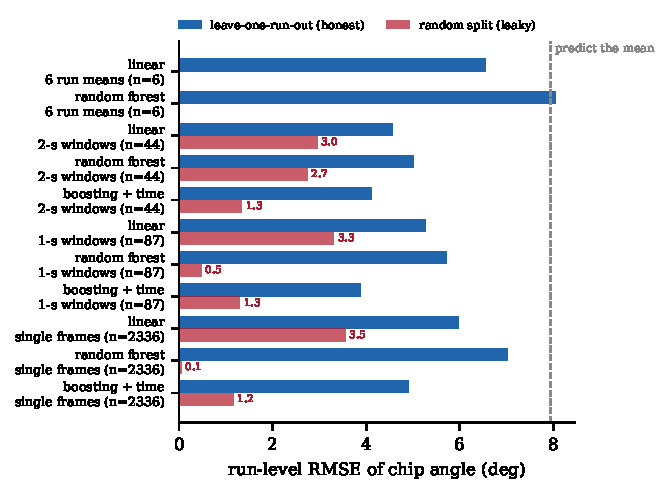
\includegraphics[width=\columnwidth]{fig14_augmentation_leakage.pdf}
\caption{Effect of cutting the six runs into many samples. Blue: honest leave-one-run-out error. Red: the same model scored with a random split of samples, which leaks the test run into training.}
\label{fig:aug}
\end{figure}

\emph{Does cutting the runs into many samples help?}
We cut each run into 2-s windows (44 samples), 1-s windows (87) or single frames (2,336) and trained on those (Fig.~\ref{fig:aug}).
Three effects have to be separated:
\begin{enumerate}
\item \emph{Cleaner target.} Window medians are a less noisy per-run target. With the linear model trained on the six run means of window medians, the error already falls from 6.6 to \SI{5.1}{\degree}.
\item \emph{More samples.} Training on the 44 windows themselves lowers it further to \SI{4.6}{\degree}. This mostly re-weights runs by their length; it adds no new cutting conditions. A random forest gains more (8.0 to \SI{5.0}{\degree}), because with five points it cannot split at all.
\item \emph{Time in the cut.} A boosted model that also knows how far into the cut a window is reaches \SIrange{3.9}{4.1}{\degree}. This is the clearest real gain, and it comes from the within-cut drift.
\end{enumerate}
Scoring the same models with a random split gives \SIrange{0.05}{3.5}{\degree}.
A random forest on single frames reaches \SI{0.05}{\degree} by recognising which run a frame came from.
These numbers are leakage, not accuracy: more samples from the same six cuts are not more cuts.

\subsection{Image models}\label{sec:res-cnn}
\begin{table}[t]
\caption{Image models, leave-one-run-out. Run RMSE: error of the predicted run mean. Slope: of predicted against measured run means (1 = no squeezing). v1/v2 trained on a Kaggle T4 GPU, v3 locally (Apple M4); one training per row.}
\label{tab:cnn}
\centering\footnotesize
\setlength{\tabcolsep}{3.5pt}
\begin{tabular}{@{}lcccc@{}}
\toprule
Model & Run RMSE & Frame MAE & $r$ & Slope \\[-1pt]
\midrule
\emph{Predict the training mean} & \emph{8.7} & \emph{9.1} & -- & 0 \\
RGB fine-tune (v1) & 8.8 & 8.8 & $-0.30$ & -- \\
Masked RGB (v2) & 7.3 & 8.3 & 0.24 & -- \\
Motion (v2, Kaggle) & 6.8 & 7.9 & 0.42 & -- \\
Motion (v2 set-up, local rerun) & \textbf{5.8} & 8.0 & \textbf{0.65} & 0.28 \\
Histogram + ridge (no CNN) & 6.7 & 8.5 & 0.49 & 0.14 \\
Motion + rotate all channels & 6.7 & 8.0 & 0.44 & 0.25 \\
Motion + rotate motion only & 6.3 & 7.9 & 0.59 & 0.37 \\
5-frame clip + rotate all & 6.4 & \textbf{7.4} & 0.58 & \textbf{0.38} \\
\bottomrule
\end{tabular}
\end{table}

\begin{figure*}[t]
\centering
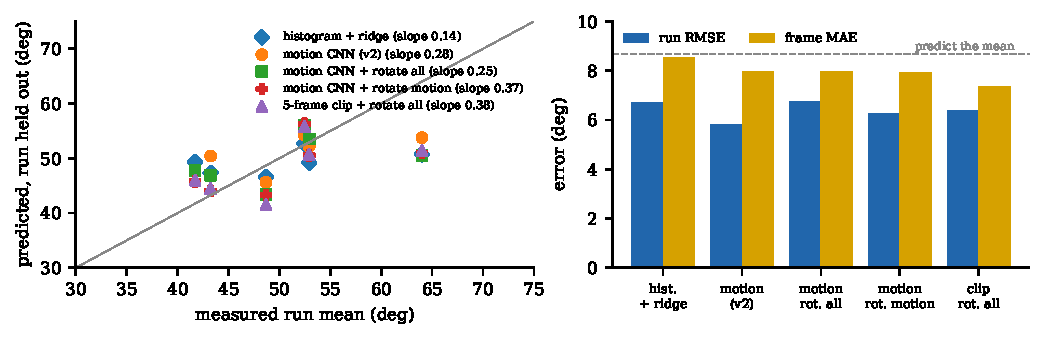
\includegraphics[width=0.85\textwidth]{fig15_cnn_v3.pdf}
\caption{Image models with the run held out. Left: predicted against measured run mean; all models are squeezed towards the middle (slopes 0.14--0.38). Right: errors; the dashed line is predicting the training mean.}
\label{fig:cnn}
\end{figure*}

Table~\ref{tab:cnn} and Fig.~\ref{fig:cnn} summarise three generations of image models.
The first network (RGB) learned which clip a frame came from rather than the chips: it was no better than the mean and anti-correlated with the truth.
Removing the static background (masked RGB, motion input) fixed most of that.

The new v3 experiments targeted the remaining problem: every model is squeezed towards the middle of the narrow training range.
The label-changing rotation, applied to the whole crop, did not help (run RMSE \SI{6.7}{\degree}, slope 0.25).
A likely reason is that the bar and the tool rotate with the chips, so the network can read $\delta$ from the tilted bar edge instead of from the chips.
Rotating only the two motion channels, with the grey image held still, closes that loophole.
It raised the slope from 0.28 to 0.37 and the correlation from 0.44 to 0.59 compared with rotating everything.
Stacking five frames gave the lowest frame error (\SI{7.4}{\degree}) and the highest slope (0.38).

These differences should not be over-read.
The same motion set-up trained twice (Kaggle and local) gave 6.8 and \SI{5.8}{\degree}, so differences under about \SI{1}{\degree} are within training noise, and each row is a single training.
No image model clearly beats the two-input linear model on run means (\SI{6.6}{\degree}).
A random split leaks here too: scored on a random fifth of frames, the rotated motion CNN reaches a frame MAE of \SI{5.0}{\degree} against \SI{8.0}{\degree} under LORO.
The useful conclusion is about the input, not the architecture.
Image models need to see motion, not the scene, and they cannot learn a range of angles that the training cuts do not contain.

\subsection{Earlier footage (out of domain)}\label{sec:res-old}
\begin{figure*}[t]
\centering
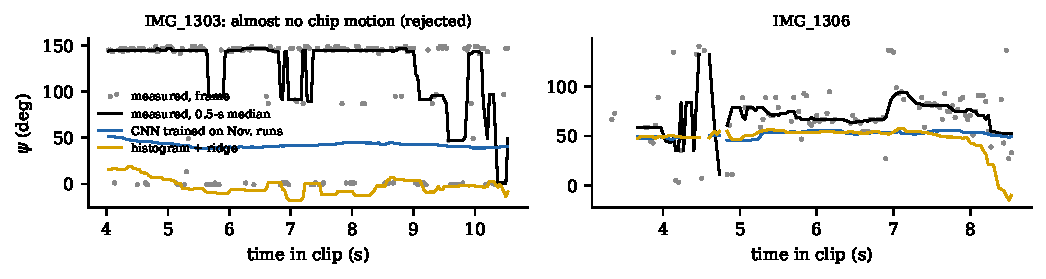
\includegraphics[width=0.85\textwidth]{fig16_old_clips.pdf}
\caption{Out-of-domain test on October footage (different part and operation, settings unknown; 60 frames/s sub-sampled to 30). Black: hand-crafted measurement. Blue and yellow: models trained on the six November runs. In IMG\_1303 there is almost no chip motion in the measuring ring, and the measurement locks on the outline of the insert.}
\label{fig:old}
\end{figure*}

The October clips were filmed while zooming in and out.
We found the stretches of constant zoom automatically: feature matching (ORB) between frames 0.2\,s apart gives the frame-to-frame scale, and stretches that stay within $\pm4\%$ were kept.
These stretches last 4.6--\SI{37}{s} in the six original-quality clips.
The compressed copies of the same footage could not be read in our environment and were not used.
Two clips most similar to the November view (looking down on the insert and the bar) were calibrated by hand: tip, feed axis, and a scale that makes the insert as large in pixels as in November.

The tracker held on 196 of 196 and 135 of 157 frames.
In IMG\_1306 the measured ejection direction is about \SI{71}{\degree}, higher than any November run (Fig.~\ref{fig:old}).
Neither image model followed it.
The November-trained CNN stayed at \SI{53}{\degree}, a frame error of \SI{19}{\degree} against \SI{21}{\degree} for always predicting \SI{50}{\degree}.
The histogram model did worse (\SI{25}{\degree}).
IMG\_1303 showed a failure mode of the measurement itself.
Its median chip-motion activity was only 2--5\% of the November runs, so almost no chips crossed the measuring ring, and the "angle" (\SI{145}{\degree}) is noise from the insert outline.
A minimum-activity gate (10\% of the quietest November run) rejects this clip automatically; it has been added to the analysis.
On new footage, then, the hand-crafted measurement keeps working once it is gated, while the image models trained on six runs do not transfer.

\subsection{Sound as a virtual sensor}
\begin{table}[t]
\caption{Sound sensor. rpm: harmonic-sum pitch. Feed from cut time and rpm.}
\label{tab:audio}
\centering\small
\begin{tabular}{@{}lccccc@{}}
\toprule
Run & rpm prog. & rpm sound & $t_\mathrm{cut}$ (s) & $f$ sound & Error \\
\midrule
R1 & 1581 & 1576 & 28.4 & 0.0819 & +2.4\% \\
R2 & 1681 & 1675 & 14.2 & 0.1539 & +2.6\% \\
R3 & 1717 & 1710 & 27.4 & 0.0783 & $-$2.2\% \\
R4 & 1755 & 1750 & 14.1 & 0.1483 & $-$1.1\% \\
R5 & 1836 & 1830 & 25.5 & 0.0786 & $-$1.8\% \\
R6 & 1925 & 1920 & 12.8 & 0.1495 & $-$0.3\% \\
\bottomrule
\end{tabular}
\end{table}
The microphone recovers the spindle speed within 0.3--0.4\% (Table~\ref{tab:audio}), which confirms both the G96 control and the inferred diameters.
It also gives the feed within 2.6\% on all six runs.
The level of the cutting noise follows the material removal rate ($r=0.91$ against $\log$ MRR).
Two other uses failed:
\begin{itemize}
\item Classifying the feed directly from the noise level was right on only 3 of 6 runs.
\item AE is known to respond to chip congestion \cite{dornfeld1985}, but the audible band of the phone showed no change on the tangled run (largest rise $-0.2$ robust units against up to 1.9 on clean runs). A phone microphone is not an AE sensor.
\end{itemize}

\subsection{Chip build-up alarm}
The training-free indicator raised the alarm only on R2, at \SI{18.7}{s} offline and \SI{20.1}{s} in the causal live version.
That is when the chips visibly snarl at the tool in the side view; in the ISO~3685 vocabulary the chips change from long to snarled \cite{iso10910}.
The other five runs peak at 0.4--1.35, against R2's 3.4, so any threshold between 1.4 and 3.4 separates them.
In R2 the spray spread rises first, then the moving area, then the static clutter.
This rests on a single tangle and is a demonstration, not a validated detector.

\subsection{Live demonstrator}
In replay mode the causal engine reproduces the offline median $\psi$ exactly on all six runs (55, 65, 49, 57, 49, 53\degr) and raises the alarm only on R2.
This is checked by 44 automated tests.
From frame arrival to finished state, the server needs a median of \SI{26}{ms} (95th percentile \SI{39}{ms}) and sustains 29 frames/s.
The calibration matters: moving the clicked tip by 5 or 10 px changes the median $\psi$ by up to 5 or \SI{7}{\degree}, which is as large as the model error.
The phone page has been tested only in a desktop browser with a simulated phone, not on a physical phone during a cut.

\section{Discussion}
\emph{Which angle should be measured?}
For comparison with the textbook, the chip-flow angle on the rake face is the right quantity.
It can be seen from the top only where the chip is wide enough to resolve: here, clearly at $a_p=\SI{0.9}{mm}$ and weakly below that.
For chip control and entanglement, the ejection direction is what matters, because it says where chips go.
It is also the more robust measurement with a phone.
Our data show the two are not the same: the chip starts on the insert side and is then turned forward by roughly \SIrange{65}{85}{\degree}, by up-curl, the chip breaker and contact with the shoulder.
A model of that turn, rather than a better flow-angle model, is what would predict where chips go.

\emph{Limitations.}
\begin{itemize}
\item Six runs from one session with one tool and one material; feed has two levels.
\item The run order is the same as the diameter and rpm order, so drift during the session cannot be separated from them.
\item The phone was handheld and uncalibrated.
\item The insert and material are assumed.
\item The rake-face direction is clearly measured on one run only.
\item The alarm rests on one tangle.
\item The image models are trained on a computer-vision label, not on an independent ground truth.
\end{itemize}

\emph{Next steps.}
\begin{itemize}
\item Photograph the insert to settle the nose radius and the chip breaker.
\item Use a fixed mount and 120--\SI{240}{frames/s}, which should make the streak estimator and the rake-face band usable at all depths.
\item Randomise the run order and repeat a centre point.
\item Add deliberately long-chip settings to collect more tangles.
\item Retrain the image model once about 30 runs exist.
\end{itemize}

\section{Conclusion}
A handheld phone measures the ejection direction of chips in turning reproducibly, recovers spindle speed and feed from sound, and flags chip build-up, all live.
The chip flow on the rake face, which classical theory predicts, can be separated from the ejection direction.
On the clearest run it lies on the insert side of the tip and agrees with Colwell's model for a nose radius of about \SI{1}{mm}.
The ejection direction, which matters for entanglement, is a different angle that no closed-form model predicts.
More samples cut from the same six runs help only a little, a random split reports leakage, not accuracy, and image models trained on six runs do not transfer to new footage. New cutting conditions are needed, not more copies of the old ones.

\begin{thebibliography}{10}
\bibitem{jawahir1993} I.~S. Jawahir and C.~A. van Luttervelt, ``Recent developments in chip control research and applications,'' \emph{CIRP Annals}, vol.~42, no.~2, pp.~659--693, 1993.
\bibitem{dornfeld1985} D.~A. Dornfeld and C.~S. Pan, ``A study of continuous/discontinuous chip formation using acoustic emission,'' \emph{J. Applied Metalworking}, vol.~4, pp.~18--29, 1985, doi:10.1007/BF02833673.
\bibitem{sukvittayawong1991} S.~Sukvittayawong and I.~Inasaki, ``Identification of chip form in turning process,'' \emph{JSME Int. J., Ser. III}, vol.~34, no.~4, pp.~553--560, 1991.
\bibitem{kishawy2018} H.~A. Kishawy \emph{et al.}, ``Application of acoustic emissions in machining processes: analysis and critical review,'' \emph{Int. J. Adv. Manuf. Technol.}, 2018, doi:10.1007/s00170-018-2341-y.
\bibitem{stabler1951} G.~V. Stabler, ``The fundamental geometry of cutting tools,'' \emph{Proc. Inst. Mech. Eng.}, vol.~165, 1951.
\bibitem{colwell1954} L.~V. Colwell, ``Predicting the angle of chip flow for single-point cutting tools,'' \emph{Trans. ASME}, vol.~76, pp.~199--203, 1954.
\bibitem{young1987} H.~T. Young, P.~Mathew, and P.~L.~B. Oxley, ``Allowing for nose radius effects in predicting the chip flow direction and cutting forces in bar turning,'' \emph{Proc. Inst. Mech. Eng.}, vol.~201, 1987, doi:10.1243/PIME\_PROC\_1987\_201\_108\_02.
\bibitem{evangelidis2008} G.~D. Evangelidis and E.~Z. Psarakis, ``Parametric image alignment using enhanced correlation coefficient maximization,'' \emph{IEEE Trans. Pattern Anal. Mach. Intell.}, vol.~30, no.~10, pp.~1858--1865, 2008.
\bibitem{kapoor2023} S.~Kapoor and A.~Narayanan, ``Leakage and the reproducibility crisis in machine-learning-based science,'' \emph{Patterns}, vol.~4, no.~9, 100804, 2023.
\bibitem{he2016} K.~He, X.~Zhang, S.~Ren, and J.~Sun, ``Deep residual learning for image recognition,'' in \emph{Proc. IEEE CVPR}, 2016, pp.~770--778.
\bibitem{iso10910} ISO 10910:1995, \emph{Chip control: classification chart}; ISO 3685:1993, \emph{Tool-life testing with single-point turning tools}, annex on chip forms.
\end{thebibliography}

\end{document}
